\documentclass[12pt,letterpaper]{report} % Tipo de archivo y tamaño de las letras y hoja
\usepackage[utf8]{inputenc} %Para que reconozca los acentos 
\usepackage[spanish]{babel}  %Idioma
\usepackage{graphicx} %Graficos
\usepackage{amsfonts,amssymb,amsthm,amsmath} %Para escribir simbolos
% Paquetes para el manejo de tablas, creación de filas y columnas unidas.
\usepackage{multirow} 
\usepackage{multicol} 
% Control de color en tablas muy versátil.
\usepackage[table]{xcolor}
% Para agregar al índice las refencias
\usepackage[nottoc,notlot,notlof]{tocbibind} 
% define el ancho del texto en la hoja
\setlength{\textwidth}{155mm}
% define el alto del texto en la hoja
\setlength{\textheight}{210mm}
% los márgenes pueden ser editador con
\usepackage{enumerate} %Para enumerar
\oddsidemargin=-.25cm
\usepackage{listings}


\begin{document}

\thispagestyle{empty}
\begin{center}
	Universidad Central de Venezuela\\
	Facultad de Ciencias.\\
	Departamento de Matemáticas.\\
	Postgrado en Modelos Aleatorios.\\
	
	\vspace{5cm}
	
	Análisis de Componentes Principales.
	
	\vspace{5cm}
	
	Daysi Lorena Febles Rivas.
	
	\vfill
	
	2017
\end{center}

\newpage

\chapter{Introducción}

El uso de internet y sus servicios es de gran importancia para el desarrollo de las empresas actuales, poder desarrollar herramientas que nos permitan hacer calculos y mostrar resultados para tomar decisiones es el objetivo de muchas empresas para presentar servicios que investigadores puedan aprovechar.

Esta pasantía tiene como objetivo crear una aplicación en la que se pueda aplicar la técnica estadística llamada componentes principales utilizando el programa estadístico R.

\section{Planteamiento del Problema}

Partiendo de una gran cantidad de variables relacionada con muchos individuos, en general, interesa simplificar la cantidad de variables y para ello se aplican métodos que identifiquen la relación que puede haber entre las variables y sólo quedarnos con las variables más representativas. Con este fin en mente se va estudiar el método de Análisis de Componentes Principales.

El Análisis de Componentes Principales fue diseñado para la reducción de dimensiones en problemas multivariados. La idea es describir con precisión los valores de $p$ variables por un subconjunto $q\le p$ de variables no correlacionadas e independientes capaces de explicar el conjunto de datos iniciales con una pequeña perdida de información.

Supongamos que tenemos $n$ observaciones de $p$ variables, se analiza si es posible representar adecuadamente esta información con un número menor de variables construidas como combinación lineal de las originales.

Los valores de las $p$ variables escalares en cada uno de los $n$ elementos puede representarse en una matriz $\mathbf{X}$, de dimensiones $(n \times p)$, que llamaremos matriz de datos. Denotaremos $x_{ij}$ el elemento que representa el valor de la variable escalar ${j}$ del individuo ${i}$.
$$
\mathbf{X}=\begin{bmatrix}
x_{11} & x_{12} & ... & x_{1p} \\
x_{21} & x_{22} & ... & x_{2p} \\
\vdots & \vdots &   & \vdots \\
x_{n1} & x_{n2} & ... & x_{np}
\end{bmatrix}_{n\times p}
$$

Se busca entonces una nueva matriz (con $q\le p$)
$$
\mathbf{Z}=\begin{bmatrix}
z_{11} & z_{12} & ... & z_{1q} \\
z_{21} & z_{22} & ... & z_{2q} \\
\vdots & \vdots &   & \vdots \\
z_{n1} & z_{n2} & ... & z_{nq}
\end{bmatrix}_{n\times q}
$$.

El objetivo de este trabajo es estudiar los conceptos necesarios para aplicar Análisis de componentes principales, comenzando con un estudio de Vectores, Matrices y Autovalores e Autovectores, luego con esto estudiar Análisis de Componentes Principales y como aplicarlo en el programa estadístico \textbf{R}.

Todo esto para crear una página web donde se muestren los resultados al aplicar Análisis de Componentes Principales y así sacar conclusiones, dicha aplicación se le aplicará a datos simulados basandos en una encuesta de satisfacción de una empresa de seguros y a otros datos encontrados en internet.

\section{Objetivos}
Se plantearon los siguientes objertivos generales y específicos:

\subsection{Objetivo General}
Elaborar material para aplicar Análisis de Componentes Principales a datos de una encuesta de satisfacción de una empresa de seguros.

\subsection{Objetivos Específicos}

\begin{enumerate}[1.]
	\item Estudiar teoría de Análisis de Componentes Principales y sus diversas metodologías aplicados al programa estadístico \textbf{R}.
	
	\begin{enumerate}[a)]
		\item Vectores con su implementación en \textbf{R}.
		\item Matrices con su implementación en \textbf{R}.
		\item Autovalores y Autovectores con su implementación en \textbf{R}.
		\item Análisis de Componentes Principales con su implementación en \textbf{R}.
	\end{enumerate}
	
	\item Generar datos simulados en \textbf{R} para aplicar Análisis de Componentes Principales.
	\item Crear láminas para un curso de Análisis de Componentes Principales utilizando \textbf{R}.	
	\item Presentación del curso Análisis de Componentes Principales utilizando \textbf{R}.
	\item Crear aplicación de Análisis de Componentes Principales con el paquete \textbf{\textit{Shiny}} en \textbf{R}.
	
\end{enumerate}

\section{Justificación}

Debido a los grandes avances tecnologicos cada vez se tiene más datos almacenados, a muchas empresas les gustaría tener herramientas que los ayuden, en bases a los mismos, a responder inquietudes con la meta de cumplir objetivos específicos. El Análisis de Componentes Principales es una herramienta que ayuda a disminuir la cantidad de datos que se tengan creando nuevas variables basadas en las originales que guarden igual cantidad de información que las variables originales.

El objetivo principal de esta pasantía es crear una página web que pueda generar datos del tipo de una encuesta de satisfacción y que también tenga la opción de poder introducir cualquier otro tipo de datos y que muestre los resultados al aplicarle Análisis de Componentes Principales para así sacar las conclusiones necesarias para responder las inquietudes del usuario.

\newpage

\chapter{Marco teórico}

En esta sección se presenta un estudio teórico de los temas necesarios para aplicar Análisis de Componentes Principales, comenzando con Vectores y matrices, luego Autovalores y Autovectores y finalmente con Análisis de Componentes Principales.

\section{Vectores}

Para introducir la noción de vector pensemos en un conjunto de $n$ datos numéricos de una variable, los cuales pueden representarse geométricamente asociando cada valor de la variable a una dimensión del espacio $n$ dimensional, obteniendo un punto en este espacio, entonces el vector será el que une el origen con dicho punto. 

Supongamos que tenemos una variable que consta de dos datos $(x_1,x_2)$, éste corresponde a un punto en el espacio $\mathbb{R}^2$, entonces el vector asociado a este punto será el que une el origen con dicho punto.

Generalmente los vectores se denotan de la siguiente manera:
$$
\mathbf{x}=
\begin{bmatrix} 
x_1 \\ 
x_2 \\ 
\vdots 
\\ 
x_n
\end{bmatrix}
$$

El vector $\mathbf{x}$ es un elemento del espacio de estado $\mathbb{R}^n$, donde los $x_i$ son los elementos o componentes del vector.

Ejemplo:

Veamos un vector en $\mathbb{R}^4$, el cual tiene los elementos $1,2,3,4$, entonces
$$
\mathbf{x}=
\begin{bmatrix}
1 \\ 
2 \\ 
3 \\ 
4
\end{bmatrix}
$$

Otro concepto muy utilizado es el de la longitud de un vector la cual se denomina norma cuadrática o norma. Esta representa la distancia que hay desde el punto $(0,0)$ al punto destino $(x,y)$ en $\mathbb{R}^2$.

La media de los datos es proporcional a la proyección del vector de datos sobre la dirección del vector constante.

La desviación típica es la distancia promedio entre el vector de datos sobre la dirección del vector constante.

La dependencia lineal entre dos variables se mide por la covarianza. El concepto análogo vectorial es el de producto escalar.

Cuando consideremos varios vectores, por ejemplo $p$ variables medidas sobre $n$ elementos de una población, el concepto principal es la noción de dependencia lineal. Esta establece cuántas variables distintas tenemos. Recordemos que una variable es dependiente de otras si a ella la podemos escribir como una combinación lineal de las otras variables.

Supongamos que tenemos los vectores ($p=2$ y $n=6$) siguientes
$$\mathbf{x_1}=\begin{bmatrix}1\\ 2 \\ 3 \\ 4 \\ 5 \\ 6 \end{bmatrix} \ \ \ \ \  \mathbf{x_2}=\begin{bmatrix} 2 \\ 4 \\ 6 \\ 8 \\ 10 \\ 12 \end{bmatrix}$$

Claramente estos vectores son dependientes ya que $\mathbf{x_1}=\frac{1}{2}\mathbf{x_2}$ o $\mathbf{x_2}=2\mathbf{x_1}$\\

\subsection{Definiciones y Propiedades}

\textbf{Definición:} \\

El \textit{\textbf{vector}} $\mathbf{x}$ es el segmento orientado que une el origen de coordenadas con el punto $\mathbf{x}$.

Con esta correspondencia a cada punto del espacio $\mathbb{R}^n$ le asociamos un vector.
$$
\mathbf{x}=\begin{bmatrix} x_1 \\ x_2 \\ \vdots \\ x_n\end{bmatrix}
$$

Un conjunto de números con todos los valores iguales se representará por un \textit{\textbf{vector constante}}, es decir, aquel que tiene todas sus coordenadas iguales.
$$
\mathbf{x}=\begin{bmatrix} \alpha \\ \alpha \\ \vdots \\ \alpha\end{bmatrix}
$$

La \textit{\textbf{suma o diferencia}} entre dos vectores $\mathbf{x}$, $\mathbf{y}$ ambos en $\mathbb{R}^n$, se define como un nuevo vector con componentes iguales a la suma (o diferencia) de los componente de los vectores
$$\mathbf{x}+\mathbf{y}=\begin{bmatrix} x_1 \\ x_2 \\ \vdots \\ x_n\end{bmatrix} + \begin{bmatrix} y_1 \\ y_2 \\ \vdots \\ y_n\end{bmatrix}=\begin{bmatrix} x_1+y_1\\ x_2+y_2 \\ \vdots \\ x_n+y_n\end{bmatrix}$$

La suma de vectores es asociativa y conmutativa:\\
$$(\mathbf{x}+\mathbf{y})+\mathbf{z}=\mathbf{x}+(\mathbf{y}+\mathbf{z})$$ 
$$\mathbf{x}+\mathbf{y}=\mathbf{y}+\mathbf{x}$$

El \textit{\textbf{producto de una constante por un vector}}, es un nuevo vector con componentes igual al vector inicial multiplicado por la constante.
$$\mathbf{z}=k\mathbf{x}=k \begin{bmatrix} x_1\\ x_2 \\ \vdots \\ x_n\end{bmatrix} =\begin{bmatrix} kx_1\\ kx_2 \\ \vdots \\ kx_n\end{bmatrix}$$

\textbf{Definición:} \\

El \textit{\textbf{vector traspuesto}}, el cual denotaremos por $\mathbf{x^t}$, de un vector $\mathbf{x}$ es un vector con las mismas componentes, pero escrito en fila.
$$\mathbf{x^t}=[ x_1 \  x_2 \ ... \ x_n]$$

\textbf{Definición:} \\

El \textit{\textbf{producto escalar o interno}} de dos vectores $\mathbf{x},\mathbf{y}$ y ambos en $\mathbb{R}^n$, que escribiremos por $\mathbf{x^ty}$ o $\mathbf{y^tx}$, es el escalar obtenido del producto de sus componentes:
$$\mathbf{x^ty}=\mathbf{y^tx}=\displaystyle\sum_{i=1}^n x_i y_i$$

\textbf{Definición:} \\

La \textit{\textbf{norma cuadrática}} o longitud de un vector $\mathbf{x}$, distancia que une el origen con el punto $\mathbf{x}$, es la raíz cuadrada positiva del producto escalar $\mathbf{x^tx}$:
$$\left\| \mathbf{x} \right\|=\sqrt{\mathbf{x^tx}}=\sqrt{x_1^2+x_2^2+...+x_n^2}$$

El producto escalar puede calcularse también como el producto de las normas de los vectores por el coseno del ángulo que forman. Observemos como es esto:

Suponga que tenemos el vector $\mathbf{x}=(a,c)$ y el vector $\mathbf{y}=(a,0)$ (ver figura 2.1)\\

\begin{figure}
	\caption{Vectores en el plano}
	\centering
	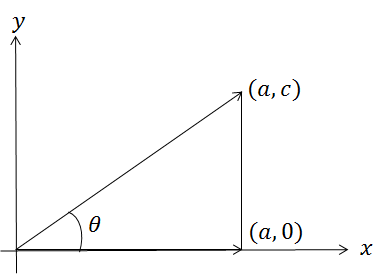
\includegraphics[width=0.4\textwidth]{img/producescal.png}
\end{figure}

El producto interno entre $\mathbf{x}$ y $\mathbf{y}$ es $$\mathbf{x^ty}=a^2+ 0c=a^2$$

La norma del vector $\mathbf{x}$ es $$\left\| \mathbf{x} \right\|=\sqrt{\mathbf{x^tx}}=\sqrt{a^2+c^2}$$

Y la norma del vector $\mathbf{y}$ es $$\left\| \mathbf{y} \right\|=\sqrt{\mathbf{y^ty}}=\sqrt{a^2+0^2}=\sqrt{a^2}=a$$

Recordemos por el teorema de pitágoras que 
$$cos(\theta)=\frac{Cateto\ Adyacente}{Hipotenusa}=\frac{CA}{H}$$

\begin{figure}
	\caption{Triángulo de Pitágoras}
	\centering
	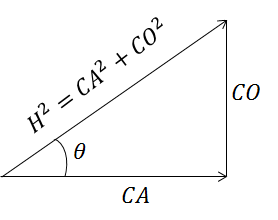
\includegraphics[width=0.4\textwidth]{img/triangulo1.png}
\end{figure}

Donde el $CA=\sqrt{a^2}=a$ (en este caso corresponde a la norma del vector $\mathbf{y}$) y $H=\sqrt{a^2+c^2}$ (longitud del vector $\mathbf{x}$), asi tenemos que
$$cos(\theta)=\frac{a}{\sqrt{a^2+c^2}}$$

Si hacemos el producto de la norma de ambos vectores con lo que obtuvimos en $cos(\theta)$ obtenemos el producto escalar entre ambos vectores, es decir:
$$\left\| \mathbf{x} \right\|\left\| \mathbf{y} \right\| cos(\theta)=a \sqrt{a^2+c^2}\frac{a}{\sqrt{a^2+c^2}}=a^2=\mathbf{x^ty}$$

Con esta idea se define \textit{\textbf{ángulo}} entre dos vectores $\mathbf{x},\mathbf{y}$ de la siguiente manera:
$$cos(\theta)=\frac{\mathbf{x^ty}}{\left\| \mathbf{x} \right\|\left\| \mathbf{y} \right\|}$$

Como $cos(\theta)\le 1$ se tiene que $|\mathbf{x^ty}| \le\left\| \mathbf{x} \right\|\left\| \mathbf{y} \right\|$, estó se conoce como la \textit{desigualdad de Caucky-Schwarz}. \\

Dos vectores son \textit{\textbf{ortogonales}}, o perpendiculares si y sólo si su producto escalar es cero.

Si dos vectores son perpendiculares forman un ángulo de $90^o$ grados, es decir $\theta=\frac{\pi}{2}$. por lo tanto si usamos la fórmula de producto interno dada, tenemos
$$cos(\theta)\left\| \mathbf{x} \right\|\left\| \mathbf{y} \right\|=cos\bigg(\frac{\pi}{2}\bigg)\left\| \mathbf{x} \right\|\left\| \mathbf{y} \right\|=0\left\| \mathbf{x} \right\|\left\| \mathbf{y} \right\|=0$$

\subsection{Conceptos estadísticos}

Para describir una variable tomamos su media. Para \textit{\textbf{describir un vector}} podemos tomar su proyeccción sobre el vector constante.

El vector constante tiene dimensión $n$, sus componentes son todas igual a $\frac{1}{\sqrt{n}}$, es decir:
$$\mathbf{c}=\begin{bmatrix} \frac{1}{\sqrt{n}} \\ \frac{1}{\sqrt{n}} \\ \vdots \\ \frac{1}{\sqrt{n}} \end{bmatrix}=\frac{1}{\sqrt{n}}\begin{bmatrix} 1 \\ 1 \\ \vdots \\ 1 \end{bmatrix}=\frac{1}{\sqrt{n}}\mathbf{1}$$

Donde la norma es $\left\| \mathbf{c} \right\| = \sum_{i=1}^n \left( \frac{1}{\sqrt{n}} \right)^2 = n\frac{1}{(\sqrt{n})^2}=\frac{n}{n}=1$

La proyección de $\mathbf{x}$ sobre el vector $c$ es 
$$\mathbf{x^tc}=\mathbf{x^t}\frac{1}{\sqrt{n}} \mathbf{1}=\sum_{i=1}^n x_i \frac{1}{\sqrt{n}}=\frac{\sum_{i=1}^n x_i}{\sqrt{n}}=\frac{n\frac{\sum_{i=1}^n x_i}{n}}{\sqrt{n}}=\sqrt{n}\bar x$$

Así el vector constante resultante de esta proyección es 
$$\mathbf{c}\sqrt{n}\bar x= \frac{1}{\sqrt{n}}\mathbf{1}\sqrt{n}\bar x=\bar x \mathbf{1}$$

La media es el escalar que define el vector obtenido al proyectar el vector datos sobre la dirección constante. 

\begin{figure}
	\caption{Media y varianza de un vector}
	\centering
	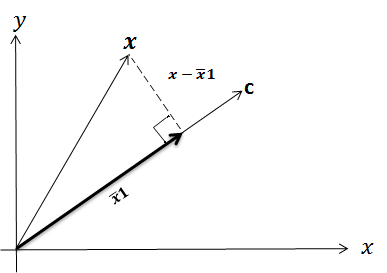
\includegraphics[width=0.6\textwidth]{img/proymed.png}
\end{figure}

La \textit{\textbf{variabilidad de los datos}} se mide por la desviación típica, que es la distancia estandarizada entre el vector de los datos y el vector constante. La norma del vector diferencia entre $\mathbf{x}-\bar x \mathbf{1}$ mide la distancia entre el vector de los datos y el vector constante.

La \textit{\textbf{norma estandarizada}} es dividir la variabilidad de los datos entre la raíz de la dimensión del vector
$$\frac{1}{\sqrt{n}}\left\| \mathbf{x}-\bar x\mathbf{1} \right\|= \sqrt{\frac{\sum_{i=1}^n (x_i-\bar x)^2}{n}}$$ 

La \textit{\textbf{covarianza}} es el producto escalar estandarizado de los dos vectores medidos en desviaciones a la media promediados. Esto mide la dependencia lineal entre dos vectores y es igual
$$\frac{1}{n}(\mathbf{x}-\bar x\mathbf{1})^t(\mathbf{y}-\bar y\mathbf{1})=\frac{\sum_{i=1}^n (x_i-\bar x)(y_i - \bar y)}{n}$$

\subsection{Dependencia Lineal}

Un conjunto de vectores $\mathbf{x_1},\mathbf{x_2},...,\mathbf{x_p}$ es linealmente dependiente si existen escalares $c_1,c_2,...,c_p$, no todos nulos tales que:
$$c_1\mathbf{x_1}+c_2\mathbf{x_2}+...+c_p\mathbf{x_p}=\mathbf{0}$$

Donde $\mathbf{0}$ es el vector nulo (todos sus componentes son cero).

El vector nulo es siempre linealmente dependiente de cualquier otro vector $\mathbf{x}$, si $\alpha\ne 0$ entonces $0\mathbf{x}+\alpha\mathbf{0}=\mathbf{0}$

Si los vectores son linealmente dependientes, podemos expresar alguno de ellos como combinación lineal del resto.

Si los vectores no son linealmente dependiente diremos que son \textit{\textbf{linealmente independientes}}. En el espacio $\mathbb{R}^p$ el número máximo de vectores linealmente
independientes es $p$.

En estadística un conjunto de vectores linealmente independientes corresponde a un conjunto de variables que no están relacionadas linealmente de forma exacta.

Dado un conjunto de $p$ valores linealmente independiente $\mathbf{x_1},\mathbf{x_2},...,\mathbf{x_p}$ en $\mathbb{R}^n$ ($p\le n$) llamaremos \textit{\textbf{espacio generado}} por esta familia de vectores al conjunto que contiene todos los vectores $\mathbf{z}$ en $\mathbb{R}^n$ que pueden expresarse como combinación lineal de éstos. Al conjunto $(\mathbf{x_1},...,\mathbf{x_p})$ se llama \textit{\textbf{familia base generadora del espacio}} o simplemente \textit{\textbf{base}} del espacio.

Supongamos que $\mathbf{z}$ pertenece a ese espacio de estados $\mathbf{z}=c_1\mathbf{x_1}+c_2\mathbf{x_2}+...+c_p\mathbf{x_p}$, de este sistema podemos agarrar las primeras $p$ coordenadas para obtener las constantes $c_1,c_2,...,c_p$ del sistema de ecuaciones.

La \textit{\textbf{dimensión}} de un espacio $E_p$ se define como el número de vectores linealmente independientes que lo generan.

Un vector $\mathbf{x}$ es ortogonal a un subespacio $E_p$ si $\mathbf{x}$ es ortogonal a todo vector de $E_p$.

Un complemento ortogonal de un subespacio $E_p$, de dimensión $p$ y lo denotaremos por $C(E_p)$, es el espacio que contiene todos los vectores ortogonales a $E_p$.

\section{Matrices}

Una matriz es un conjunto de números dispuestos en filas y columnas, que puede verse como un conjunto de vectores columnas o un conjunto de vectores filas.

\subsection{Definiciones y Propiedades}

\textbf{Definición:}

Definiremos una \textit{\textbf{matriz}} $\mathbf{A}$ de dimensiones $n \times p$ a un conjunto de $n \times p$ números reales, ordenados en $n$ filas y $p$ columnas.
$$
\mathbf{A}=\begin{bmatrix}
x_{11} & x_{12} & ... & x_{1p} \\
x_{21} & x_{22} & ... & x_{2p} \\
\vdots & \vdots &   & \vdots \\
x_{n1} & x_{n2} & ... & x_{np} 
\end{bmatrix}_{n\times p}
$$

La \textit{\textbf{matriz traspuesta}} es la matriz obtenida a traves de $\mathbf{A}$ intercambiando filas por columnas, la denotaremos por $\mathbf{A}^t$. Si $\mathbf{A}$ tiene dimensión $n \times p$ entonces $\mathbf{A}^t$ tiene dimension $p \times n$. 
$$
\mathbf{A^t}=\begin{bmatrix}
x_{11} & x_{21} & ... & x_{p1} \\
x_{12} & x_{22} & ... & x_{p2} \\
\vdots & \vdots &   & \vdots \\
x_{1p} & x_{2p} & ... & x_{pn} 
\end{bmatrix}_{p\times n}
$$
\\
\textbf{Nota}:

La traspuesta a una verifica $(\mathbf{A}^t)^t=\mathbf{A}$ \\

La \textit{\textbf{suma de dos matrices}} se define sólo cuando ambas tienen las mismas dimensiones. Cada elemento de la matriz suma se obtiene sumando los elementos correspondientes a los sumandos.
$$
\mathbf{A}+\mathbf{B}=
\begin{bmatrix}
a_{11} & a_{12} & ... & a_{1p} \\
a_{21} & a_{22} & ... & a_{2p} \\
\vdots & \vdots &     & \vdots \\
a_{n1} & a_{n2} & ... & a_{np} \\
\end{bmatrix}_{n\times p}
+
\begin{bmatrix}
b_{11} & b_{12} & ... & b_{1p} \\
b_{21} & b_{22} & ... & b_{2p} \\
\vdots & \vdots &     & \vdots \\
b_{n1} & b_{n2} & ... & b_{np} \\
\end{bmatrix}_{n\times p}
=
\begin{bmatrix}
a_{11}+b_{11} & a_{12}+b_{12} & ... & a_{1p}+b_{1p} \\
a_{12}+b_{12} & a_{22}+b_{22} & ... & a_{2p}+b_{2p} \\
\vdots & \vdots &     & \vdots \\
a_{n1}+b_{n1} & a_{n2}+b_{n2} & ... & a_{np}+b_{np} \\
\end{bmatrix}_{n\times p}
$$
\\
\textbf{Nota}:
\begin{itemize}
\item La suma es conmutativa $\mathbf{A}+\mathbf{B}=\mathbf{B}+\mathbf{A}$
\item La suma es Asociativa $(\mathbf{A}+\mathbf{B})+\mathbf{C}=A+(\mathbf{B}+\mathbf{C})$
\item $(\mathbf{A}+\mathbf{B})^t=\mathbf{B}^t+\mathbf{A}^t$
\end{itemize}

La \textit{\textbf{multiplicación de un escalar por una matriz}}, es una nueva matriz con las mismas componentes de la matriz multiplicadas por el escalar, es decir:
$$
\alpha \mathbf{A}=
\alpha\begin{bmatrix}
a_{11} & a_{12} & ... & a_{1p} \\
a_{21} & a_{22} & ... & a_{2p} \\
\vdots & \vdots &     & \vdots \\
a_{n1} & a_{n2} & ... & a_{np} \\
\end{bmatrix}_{n\times p}
=
\begin{bmatrix}
\alpha a_{11} & \alpha a_{12} & ... & \alpha a_{1p} \\
\alpha a_{21} & \alpha a_{22} & ... & \alpha a_{2p} \\
\vdots & \vdots &     & \vdots \\
\alpha a_{n1} & \alpha a_{n2} & ... & \alpha a_{np} \\
\end{bmatrix}_{n\times p}
$$
\\

El \textit{\textbf{producto matricial}} entre dos matrices $\mathbf{A}$ y $\mathbf{B}$, se denotará por $\mathbf{A}\mathbf{B}$ y solo se definirá cuando el número de columnas de la matriz $\mathbf{A}$ es igual al número de filas de la matriz $\mathbf{B}$. Si $\mathbf{A}$ es $n \times p$ y $\mathbf{B}$ es $p \times h$, entonces el producto de estas dos matrices será otra matriz de dimensión $n \times h$ y los elementos correspondientes a la $(i,j)$ posición serán iguales a $\sum_{m=1}^{p} a_{im}b_{mj}$.

Esto es lo mismo que decir que el componente $(i,j)$ es el producto del vector que corresponde a la fila $i$ de la matriz $\mathbf{A}$ con el vector de la columna $j$ del vector $\mathbf{B}$ 
$$
C_{ij}=\begin{bmatrix} a_{i1} & a_{i2} & ... & a_{ip} \end{bmatrix} \begin{bmatrix} b_{1j}\\ b_{2j} \\ \vdots \\ b_{pj}\end{bmatrix} =\sum_{m=1}^{p} a_{im}b_{mj}
$$
\\
\textbf{Nota}:

El producto de matrices no es en general conmutativo ya que si $\mathbf{A}\mathbf{B}$ existe el producto $\mathbf{B}\mathbf{A}$ puede no existir. En caso de que exista es en general distinto de $\mathbf{A}\mathbf{B}$
\\

En particular el producto de una matriz $\mathbf{A}$ de dimensiones $(n \times p)$ por un vector $x$ de $(p \times 1)$, $\mathbf{Ax}$, será un nuevo vector de dimensión $(n \times 1)$ cuyas componentes son el producto interno de las filas de $\mathbf{A}$ con el vector $x$.
$$
\mathbf{A}x=
\begin{bmatrix}
a_{11} & a_{12} & ... & a_{1p} \\
a_{21} & a_{22} & ... & a_{2p} \\
\vdots & \vdots &     & \vdots \\
a_{n1} & a_{n2} & ... & a_{np} \\
\end{bmatrix}_{n\times p}
\begin{bmatrix} x_1 \\ x_2 \\ \vdots \\ x_p\end{bmatrix}_{p\times 1}
= \begin{bmatrix} x_1a_{11}+x_2a_{12}+...+x_pa_{1p} \\ x_1a_{21}+x_2a_{22}+...+x_pa_{2p} \\ \vdots \\ x_1a_{n1}+x_2a_{n2}+...+x_p a_{np}\end{bmatrix}_{n\times 1}
$$
\\

La \textit{\textbf{matriz identidad}} de dimensión $n$, $\mathbf{I}_n$ es la matriz de dimensiones  $(n \times n)$ que tiene 1 en los elementos de la diagonal y 0 en el resto de sus elementos.  
$$
\mathbf{I}=
\begin{bmatrix}
1 & 0 & ... & 0 \\
0 & 1 & ... & 0 \\
\vdots   & \vdots &  \ddots & \vdots \\
0 & 0 & ... & 1 \\
\end{bmatrix}_{n\times n}
$$
\\
\textbf{Nota}:
\begin{itemize}
\item $\mathbf{A}(\mathbf{B}+\mathbf{C})=\mathbf{A}\mathbf{B}+\mathbf{A}\mathbf{C}$
\item $(\mathbf{A}\mathbf{B})^t=\mathbf{B}^t\mathbf{A}^t$ 
\item $\mathbf{A}\mathbf{I}=\mathbf{I}\mathbf{A}=\mathbf{A}$
\end{itemize}

El \textit{\textbf{rango de una matriz}}, indica el número máximo de filas o columnas linealmente independientes que contiene la matriz.

En una matriz de dimensión $(n \times p)$. Suponiendo que $n>p$ el máximo de número de vectores linealmente independientes es $p$, en efecto si consideramos los vectores formados por las $p$ columnas, estos estan en $\mathbb{R}^n$ , entonces solo hay $p$ que pueden ser linealmente independientes. Si consideramos los $n$ vectores filas estos estan en $\mathbb{R}^p$ y el máximo número de vectores independientes es $p$. Por lo tanto, el rango máximo de la matriz es $p$, y cuando esto ocurre decimos que la matriz es de rango completo. 

De la definición el rango de una matriz y el de su traspuesta es el mismo.
\\
Si denotamos el rango de una matriz $\mathbf{A}$ por $rg(\mathbf{A})$ se verifica lo siguiente:
\begin{itemize}
\item $rg(\mathbf{A}_{n\times p})\le min(n,p)$ el rango es menor o igual que el menor de $n$ y $p$.
\item Si $rg(\mathbf{A}_{n\times p})=min(n,p)$ se dice que $\mathbf{A}$ es de rango completo. 
\item $rg(\mathbf{A}+\mathbf{B}) \le rg(\mathbf{A}) + rg(\mathbf{B})$
\item $rg(\mathbf{AB}) \le min(rg(\mathbf{A}),rg(\mathbf{B}))$
\item $rg(\mathbf{A}^t\mathbf{A})=rg(\mathbf{A}\mathbf{A}^t)=rg(\mathbf{A})$
\end{itemize}

En estadística el rango de una matriz nos indica la dimensión real para presentar los datos, o  el número real de variables distintas que disponemos. Con el rango podemos reducir el número de variables sin pérdida de información.

Una \textit{\textbf{matriz es cuadrada}} si $p=n$, y este número se denomina orden de la matriz.
$$
\mathbf{A}=
\begin{bmatrix}
a_{11} & a_{12} & ... & a_{1n} \\
a_{21} & a_{22} & ... & a_{2n} \\
\vdots & \vdots &     & \vdots \\
a_{n1} & a_{n2} & ... & a_{nn} \\
\end{bmatrix}_{n\times n}
$$

El rango máximo de una matriz cuadrada de orden $n$ es $n$. Cuando el rango es menor que $n$ una fila o columna es combinación lineal de las demás y decimos que la matriz es \textit{\textbf{singular}}.

Diremos que una \textit{\textbf{matriz $\mathbf{A}$ es simétrica}} si $\mathbf{A}^t=\mathbf{A}$.

Una clase importante de matrices cuadradas y simétricas son las \textit{\textbf{matrices diagonales}}, que tienen únicamente terminos no nulos en la diagonal principal, un ejemplo de estas matrices es la matriz identidad definida anteriormente.

Los productos $\mathbf{A}^t\mathbf{A}$ y $\mathbf{A}\mathbf{A}^t$ conducen a matrices simétricas.

Una \textit{\textbf{matriz triangular superior}} es una matriz cuadrada donde todas las componentes que estan por debajo de la diagonal principal son iguales a cero. 
$$
\mathbf{A}=
\begin{bmatrix}
a_{11} & a_{12} & ... & a_{1n} \\
0 & a_{22} & ... & a_{2n} \\
\vdots & \vdots & \ddots & \vdots \\
0 & 0 & ... & a_{nn} \\
\end{bmatrix}_{n\times n}
$$

Una matriz es \textit{\textbf{estrictamente triangular superior}} si los componentes de la diagonal y debajo de estos son iguales a cero.
$$
\mathbf{B}=
\begin{bmatrix}
0 & b_{12} & ... & b_{1n} \\
0 & 0 & ... & b_{2n} \\
\vdots & \vdots & \ddots & \vdots \\
0 & 0 & ... & 0 \\
\end{bmatrix}_{n\times n}
$$

Analogamente se tiene una \textit{\textbf{matriz triangular inferior}}, es esto caso sus componentes por encima de la diagonal principal son ceros.
\\

\textbf{Determinante}
\\

Dada una matriz $\mathbf{A}$ cuadrada de orden $n$, se denomina \textit{\textbf{determinante de la matriz}}, y lo denotaremos por $|\mathbf{A}|$, al escalar obtenido mediante la suma de todos los productos de $n$ elementos de la matriz $a_{1i_1}a_{2i_2}...a_{ni_n}$, que podemos formar de manera que en cada producto aparezca una vez un elemento de cada fila y uno de cada columna. Cada término tiene además un signo, que depende del número de cambios entre dos subíndices consecutivos, que es necesario para poner los subíndices $i_1 i_2 ... i_n$ de este término en el orden natural $1,2,...,n$. Escribiremos:
$$|\mathbf{A}|=\sum (-1)^r a_{1i_1}a_{2i_2}...a_{ni_n}$$
Donde el sumatorio está extendido a las $n!$ permutaciones de los segundos índices. Los índices $i_1,i_2,...,i_n$ son una permutación de los números $1,2,...,n$ y $r$ es el número de cambios entre dos subíndices necesario para ponerlos en el orden $1,2,...,n$.

Si la matriz $\mathbf{A}$ es una matriz de $(2 \times 2)$
$$
\mathbf{A}=
\begin{bmatrix}
a_{11} & a_{12} \\
a_{21} & a_{22} \\
\end{bmatrix}
$$

Los determinantes tienen las propiedades siguientes, si $\mathbf{A}$ es una matriz de orden $n$:
\begin{itemize}
\item $|\lambda \mathbf{A}|=\lambda^n|\mathbf{A}|$
\item $|\mathbf{A}|^t=|\mathbf{A}|$
\item Si $\mathbf{A}$ y $\mathbf{B}$ son dos matrices cuadradas $|\mathbf{A}\mathbf{B}|=|\mathbf{A}||\mathbf{B}|$
\item Si permutamos dos filas o dos columnas entre sí, el determinante cambia sólo el signo.
\item Si una fila (columna) de una matriz es combinanción lineal de las restantes filas (columnas), lo que supone que su rango es menor que $n$, la matriz se denomina \textit{\textbf{singular}} y su determinante es cero.	
\end{itemize}

La \textit{\textbf{traza}} de una matriz cuadrada es la suma de los elementos de la diagonal principal de la matriz.
$$tr(\mathbf{A})=\sum_{i=1}^{n}a_{ii}$$

Se obtiene que:
\begin{itemize}
\item  $tr(\mathbf{A}+\mathbf{B})=tr(\mathbf{A})+tr(\mathbf{B})$
\item $tr(\lambda\mathbf{A})=\lambda tr(\mathbf{A})$
\item $tr(\mathbf{A}\mathbf{B}\mathbf{C})=tr(\mathbf{B}\mathbf{C}\mathbf{A})=tr(\mathbf{C}\mathbf{A}\mathbf{B})$, en el caso donde los productos esten definidos.
\item Si la matriz $\mathbf{C}$ es simétrica entonces $tr(\mathbf{C}^2)=tr(\mathbf{C}\mathbf{C})=\sum_{i=1}^{n}\sum_{j=1}^{n}\mathbf{C}_{ij}^2$
\end{itemize} 

\textbf{Forma cuadrática} \\

Transformemos un vector $\mathbf{x}$ mediante una transformación lineal $\mathbf{y}=\mathbf{Bx}$ la norma al cuadrado del nuevo vector será:
$$\mathbf{y^ty}=\mathbf{x^tB^tBx}=\mathbf{x^tAx}\ge 0$$

Donde $\mathbf{A}=\mathbf{B^tB}$ es una matriz cuadrada y simétrica.

Llamaremos \textit{\textbf{forma cuadrática}} a una expresión escalar del tipo $\mathbf{x^t\mathbf{A}x}$ donde $\mathbf{x}$ es un vector y $\mathbf{A}$ es una matriz cuadrada y simétrica. Su expresión general es:
$$\sum_{i=1}^{n} a_{ii}x_{i}^2 + 2\sum_{i=1}^{n}\sum_{j=i+1}^{n}a_{ij}x_{i}x_{j}$$

La matriz $\mathbf{A}$ es \textit{\textbf{semidefinida positiva}} si cualquier forma cuadrática formada a partir de ella es un número no negativo para cualquier vector $\mathbf{x}\ne 0$.

Si la forma cuadrática es siempre un número positivo diremos que la matriz $\mathbf{A}$ es \textit{\textbf{definida positiva}}. \\

\textbf{Inversa}
\\

Dada una matriz $\mathbf{A}$ cuadrada de orden $n$, no singular, definimos su \textit{\textbf{inversa}} $\mathbf{A}^{-1}$ como una matriz de orden $n$ tal que:
$$\mathbf{A}\mathbf{A}^{-1}=\mathbf{A}^{-1}\mathbf{A}= \mathbf{I}$$

Escribiendo $\mathbf{A}$ con vectores filas $\mathbf{a_{i}}$ y a $\mathbf{A}^{-1}$ con vectores columnas $\mathbf{b_{i}}$ tales que:
$$
\mathbf{A}\mathbf{A}^{-1}=\begin{bmatrix} \mathbf{a_{1}^t}\\ \mathbf{a_{2}}^t \\ \vdots \\ \mathbf{a_{n}}^t\end{bmatrix}_{n\times 1} \begin{bmatrix} \mathbf{b_{1}} & \mathbf{b_{2}} & ... & \mathbf{b_{n}} \end{bmatrix}_{1\times n}= \begin{bmatrix} \mathbf{a_{1}^tb_{1}} & \mathbf{a_{1}^tb_{2}} & ... & \mathbf{a_{1}^tb_{n}}\\  \mathbf{a_{2}^tb_{1}} & \mathbf{a_{2}^tb_{2}} & ... & \mathbf{a_{2}^tb_{n}} \\ \vdots & \vdots & \ddots & \vdots \\  \mathbf{a_{n}^tb_{1}} & \mathbf{a_{n}^tb_{2}} & ... & \mathbf{a_{n}^tb_{n}}  \end{bmatrix}_{n\times n}=
\begin{bmatrix}
1 & 0 & ... & 0 \\
0 & 1 & ... & 0 \\
\vdots   & \vdots &  \ddots & \vdots \\
0 & 0 & ... & 1 \\
\end{bmatrix}_{n\times n}
$$

Obervando esto último podemos decir que la matriz inversa es tal que sus vectores columna son ortogonal a los vectores filas, esto es $\mathbf{a_{i}^tb_{j}}=0$ cuando $i\ne j$, y es uno cuando $i=j$.

La inversa de una matriz tiene las siguientes propiedades:
\begin{itemize}
\item $(\mathbf{AB})^{-1}=\mathbf{B}^{-1}\mathbf{A}^{-1}$
\item $(\mathbf{A}^{t})^{-1}=(\mathbf{A}^{-1})^{t}$
\item $|\mathbf{A}^{-1}|=|\mathbf{A}|^{-1}$
\item Si $\mathbf{A}$ es simétrica también lo es $\mathbf{A}^{-1}$
\end{itemize}

\textbf{Derivadas matriciales} \\

\textbf{Definición:}

Dada una función $f$ que depende de $n$ variables $x_1,...,x_n$, que pueden considerarse componentes de un vector $\mathbf{x}$, la derivada de $f$ respecto a $\mathbf{x}$ es un vector cuyos componentes son la derivada de $f$ respecto a cada componente de $\mathbf{x}$.

\begin{itemize}
\item Si $f=\mathbf{a^tx}$ tendremos $\frac{\partial(\mathbf{a^tx})}{\partial \mathbf{x}}=\mathbf{a}$.
\item Si $f=\mathbf{x^tAx}$ donde $\mathbf{A}$ es cuadrada y simétrica, entonces $\frac{\partial(\mathbf{x^tAx})}{\partial \mathbf{x}}=\mathbf{2Ax}$.
\end{itemize}

\textbf{Definición:}

Dada una función $f$ que depende de $np$ variables $x_{11},...,x_{np}$, que son los componentes de una matriz rectangular $n\times p$, $\mathbf{X}$, la derivada de $f$ respecto a $\mathbf{X}$ se define como una matriz cuyos componentes son la derivada de $f$ respecto a cada componente de $\mathbf{X^t}$. La derivada es una matriz $p\times n$ con las dimensiones de $\mathbf{X^t}$.

\begin{itemize}
\item  Si $f=\mathbf{a^tXb}$ tendremos $\frac{\partial (\mathbf{a^tXb})}{\partial \mathbf{X}}=\mathbf{ba^t}$.
\item  Si $f=\mathbf{a^tX^tXb}$ entonces $\frac{\partial (\mathbf{a^tX^tXb})}{\partial \mathbf{X}}=(\mathbf{ab^t}+\mathbf{ba^t})\mathbf{X^t}$.
\end{itemize}

\textbf{Definición:}

Dado un vector $\mathbf{y}$ cuyos componentes son funciones $f_i$ de un vector de variables $\mathbf{x^t}=(x_1,...,x_n)$ definamos la derivada de $\mathbf{y}$ con respecto a $\mathbf{x}$ como la matriz cuyas columnas son las derivadas de las componentes $f_i$ respecto a $\mathbf{x}$, es decir:
$$\mathbf{y^t}=(f_1(\mathbf{x}),...,f_n(\mathbf{x}))$$

Entonces

$$\frac{\partial \mathbf{y}}{\partial \mathbf{x}}=\begin{bmatrix} \frac{\partial f_1(\mathbf{x})}{\partial \mathbf{x}},...,\frac{\partial f_n(\mathbf{x})}{\partial \mathbf{x}}\end{bmatrix}= 
\begin{bmatrix}
\frac{\partial f_1(\mathbf{x})}{\partial x_1} & \frac{\partial f_2(\mathbf{x})}{\partial x_1} & ... & \frac{\partial f_n(\mathbf{x})}{\partial x_1} \\
\vdots   & \vdots &   & \vdots \\
\frac{\partial f_1(\mathbf{x})}{\partial x_n} & \frac{\partial f_2(\mathbf{x})}{\partial x_n} & ... & \frac{\partial f_n(\mathbf{x})}{\partial x_n} 
\end{bmatrix} $$

A esta matriz se le denomina \textit{\textbf{matriz Jacobiana}}.

Si $\mathbf{y}=\mathbf{Ax}$, donde $\mathbf{A}$ es una matriz cualquiera $\frac{\partial \mathbf{Ax}}{\partial \mathbf{x}}=\mathbf{A^t}$.

\section{Autovalores y Autovectores propios}

También llamados valores y vectores propios. 

Los valores propios son las medidas básicas de tamaño de una matriz, que no se ven alteradas si hacemos un cambio de coordenadas que equivale a una rotación de los ejes.

Los vectores propios representan las direcciones características de la matriz y no son invariantes. 

\subsection{Deficiones y propiedades}

Llamaremos \textit{\textbf{vectores propios}} de una matriz cuadrada de orden $n$ a aquellos vectores cuya dirección no se modifica al transformarlos mediante una matriz. Por lo tanto $\mathbf{u}$ es un vector propio de la matriz $\mathbf{A}$ si verifica que:

$$\mathbf{Au}=\lambda\mathbf{u} \qquad (1)$$ 

Donde $\lambda$ es un escalar, que se denomina valor propio de la matriz. En esta relación suponemos $\mathbf{u} \ne \mathbf{0}$. Si $\mathbf{u}$ es un vector propio de $\mathbf{A}$ y multiplicamos por un escalar $a \ne 0$ en la ecuación $(1)$, tenemos que $a\mathbf{u}$ también es un vector propio de $\mathbf{A}$, para evitar esta indeterminación supondremos que los vectores propios estan normalizados de manera que $\left\| \mathbf{u} \right\|=1$.

Para calcular el vector propio podemos escribir la ecuación anterior como:
$$
\begin{array}{rl}
\mathbf{Au} = & \lambda\mathbf{u}\\
\mathbf{Au}- \lambda\mathbf{u} = & 0\\
(\mathbf{A}- \lambda\mathbf{I})\mathbf{u} = & 0
\end{array}
$$

Que es un sistema de ecuaciones homogéneo que tendrá solución no nula si y sólo si la matriz del sistema $(\mathbf{A}- \lambda\mathbf{I})$ es singular.

Este sistema tiene solución no nula si se verifica que:
$$|\mathbf{A}- \lambda\mathbf{I}|=0$$

Esta ecuación se denomina la \textit{\textbf{ecuación característica}} de la matriz. Es una ecuación polinómica en $\lambda$ de orden $n$ y sus $n$ raices se denominan \textit{\textbf{valores propios}} de la matriz.

A cada valor propio distinto de la matriz cuadrada podemos asociarle un único vector propio que satisface $(1)$. Como la matriz es singular, existen infinitas soluciones, ya que si $\mathbf{u}$ es solución también lo es $a\mathbf{u}$, lo que resolvemos tomando el vector de norma uno.

Los valores propios de una matriz tienen las propiedades siguientes:
\begin{itemize}
\item[1] Si $\lambda$ es un valor propio de $\mathbf{A}$, entonces $\lambda^r$ es un valor propio de $\mathbf{A}^r$. En particular si $\mathbf{A}$ es no singular, $\lambda \ne 0$ y $\lambda^{-1}$ es un valor propio de $\mathbf{A}^{-1}$.

Si $\mathbf{Au}=\lambda\mathbf{u}$, multiplicando por $\mathbf{A}$ tenemos $\mathbf{A^2u}=\lambda^2\mathbf{u}$ y asi sucesivamente.

\item[2] Los valores propios de una matriz y de su traspuesta son los mismos.

Sea $\mathbf{Au}=\lambda \mathbf{u}$ y $\mathbf{A^t v}=\mu \mathbf{v}$ multiplicando la primera ecuación por $\mathbf{v}^t$ y la segunda por $\mathbf{u}^t$ tenemos $\mathbf{v^t A u}=\lambda \mathbf{v^tu}$ y $\mathbf{u^t A^t v}=\mu \mathbf{u^t v}$ en este caso tenemos que de estas dos últimas ecuaciones el primer termino es el mismo por lo tanto $\lambda \mathbf{v^tu}=\mu \mathbf{u^t v}$ lo que implica $\lambda=\mu$

\item[3] La suma de los valores propios de $\mathbf{A}$ es igual a la traza $tr(\mathbf{A})=\sum \lambda_{i}$

\item[4] El producto de los valores propios de $\mathbf{A}$ es igual al determinante $|\mathbf{A}|=\prod \lambda_{i}$

\item[5] Si $\mathbf{P}$ es no singular, las matrices $\mathbf{A}$ y $\mathbf{P}^{-1}\mathbf{A}\mathbf{P}$ tienen los mismos valores propios.

Si $\mathbf{Au}=\lambda \mathbf{u}$ multiplicando por la izquierda $\mathbf{P^{-1}}$ y por la derecha $\mathbf{P}$ tenemos $\mathbf{P^{-1}APu}=\lambda \mathbf{P^{-1}Pu}=\lambda \mathbf{u}$ asi las matrices tienen los mismos valores propios.

\item[6] Las matrices $\mathbf{A}$ y $\mathbf{A\pm I}$ tienen los mismos vectores propios y si $\lambda$ es un valor propio de $\mathbf{A}$, $\lambda \pm 1$ es un valor propio de $\mathbf{A\pm I}$.

Si $\mathbf{Au}=\lambda \mathbf{u}$ entonces $\mathbf{Au+ Iu}=\lambda \mathbf{u}+ \mathbf{u}$ es decir $(\mathbf{A+ I})\mathbf{u}=(1+\lambda) \mathbf{u}$ por otro lado $|\mathbf{A}-\lambda \mathbf{I}|=0$ entonces también $|\mathbf{A+I-I}-\lambda \mathbf{I}|=|(\mathbf{A+I})+(1-\lambda) \mathbf{I}|=0$

\item[7] Las matrices cuadradas $\mathbf{ABC}$, $\mathbf{BCA}$ y $\mathbf{CAB}$ , donde las matrices $\mathbf{A}$, $\mathbf{B}$ y $\mathbf{C}$ son generales con la condición de que los productos existan, tienen los mismos valores propios no nulos.

\item[8] Si $\mathbf{A}$ es triangular los valores propios son los elementos de la diagonal.
\end{itemize}

\textbf{Valores propios y vectores propios de matrices simétricas} \\

En las matrices simétricas los valores propios son siempre reales los vectores propios son ortogonales.

Supongamos que tenemos dos valores y vectores propios entonces: 

$\mathbf{Au_{i}}=\lambda_{i}\mathbf{u_{i}}$ y  $\mathbf{Au_{j}}=\lambda_{j}\mathbf{u_{j}}$ multiplicando la primera ecuación por $\mathbf{u_{j}}^t$ y la segunda por $\mathbf{u_{i}}^t$ lo que implica que  $\lambda_{i}\mathbf{u_{j}^tu_{i}}=\lambda_{j}\mathbf{u_{i}^tu_{j}}$ ahora como $\lambda_{i} \ne \lambda_{j}$ sólo serán iguales si $\mathbf{u_{j}^tu_{i}}=\mathbf{u_{i}^tu_{j}}=0$, es decir son ortogonales.

Los valores propios de una matriz simétrica representan las magnitudes de los ejes del elipsoide con centro en el origen y determinado por los extremos de los vectores. Los vectores propios indican las direcciones de estos ejes principales.\\

\textbf{Descomposición en valores singulares} \\

Toda matriz rectangular $\mathbf{A}$ de dimensiones $(n\times p)$ y de rango $r$ puede expresarse como el producto de tres matrices, dos de ella ortogonales y la tercera diagonal. La descomposición es:
$$\mathbf{A}=\mathbf{UD^{1/2}V^t}$$
Donde $\mathbf{U}$ es $(n \times r)$, $\mathbf{D}^{1/2}$ es $(r \times r)$ y $\mathbf{V}^t$ es $(r \times p)$.

La matriz $\mathbf{D}^{1/2}$ es diagonal y contiene las raices cuadradas de los valores propios no nulos de las matrices $\mathbf{AA^t}$ o $\mathbf{A^tA}$ que son positivos, estos términos diagonales se denominan los \textit{valores singulares} de la matriz $\mathbf{A}$.

La matriz $\mathbf{U}$ contiene en columnas los vectores propios de norma unidad asociados a los valores propios no nulos de $\mathbf{AA^t}$.

La matriz $\mathbf{V}$ contiene en columna los vectores propios en unidad asociados a valores propios no nulos de $\mathbf{AA^t}$.

Las columnas de $\mathbf{U}$ son ortogonales entre sí y también lo serán las de $\mathbf{V}$.

Observemos que si la matriz $\mathbf{U}$ contiene los vectores propios de norma unidad de $\mathbf{A^tA}$  entonces como $\mathbf{A^tAu_{i}}=\lambda_{i}\mathbf{u_{i}}$ multiplicando por $\mathbf{A^t}$ tenemos $\mathbf{(A^tA)A^tu_{i}}=\lambda_{i}\mathbf{A^tu_{i}}=\lambda_{i}\mathbf{w_{i}}$ y el vector $\mathbf{w_{i}}=\mathbf{A^tu_{i}}$ es un vector propio de $\mathbf{A^tA}$. Sin embargo este vector propio no tiene norma unidad ya que $\mathbf{w_{i}^t w_{i}}=\mathbf{u_{i}^tAA^tu_{i}}=\lambda_{i}$.

Los vectores propios de $\mathbf{A^tA}$ de norma unidad vienen dados por $\mathbf{V}=\mathbf{A^t U D^{-1/2}}$
$$ 
\begin{array}{rl}
\mathbf{A}= & \mathbf{U}\mathbf{D}^{1/2}(\mathbf{A}^t \mathbf{U} \mathbf{D}^{-1/2})^t\\
= & \mathbf{UD}^{1/2}(\mathbf{D}^{-1/2})^t\mathbf{U}^t(\mathbf{A}^t)^t\\
= & \mathbf{UD}^{1/2}(\mathbf{D}^{-1/2})^t\mathbf{U}^t \mathbf{A}\\
= & \mathbf{UI}\mathbf{U}^t \mathbf{A}\\
= & \mathbf{I} \mathbf{A}\\
= & \mathbf{A}\\
\end{array}
$$

\section{Análisis de Componentes Principales}

El Análisis de Componentes Principales es el primer paso para identificar las posibles variables latentes, o no observadas que generan los datos. 

Al mismo tiempo, permite transformar las variables originales, en general correlacionadas, en nuevas variables incorrelacionadas, facilitando la interpretación de los datos.

Recordemos que la variabilidad respecto a la media se mide habitualmente calculando la varianza, o su raíz cuadrada, la desviación típica. 

Un estimador de la varianza es $\frac{1}{n}\mathbf{\tilde{X}^t\tilde{X}}$ y el estimador insesgado es $\frac{1}{n-1}\mathbf{\tilde{X}^t\tilde{X}}$, donde $\mathbf{\tilde{X}}$ es la matriz resultante de la resta de la matriz de datos $\mathbf{X}$ con la matriz de medias $\bar{\mathbf{X}}$.

La relación lineal entre dos variables se mide mediante la covarianza y se cálcula de la forma siguiente:
$$
\begin{array}{rl}
& \mbox{si }i\ne j  \to \ S_{ij} = \frac{1}{n}\sum_{k=1}^{n}(x_{kj}-\bar x_{j})(x_{ki}-\bar x_{i}) \\
& \mbox{si }i=j \to S_{i}^2 = \frac{1}{n}\sum_{k=1}^{n}(x_{ki}-\bar x_{i})^2
\end{array}
$$

Ésta mide la dependencia lineal entre las variables.

Para definir la matriz de varianzas y covarianzas definiremos primero la matriz de medias, de la siguiente manera:
$$
\bar{\mathbf{X}}=\begin{bmatrix}
\bar{x}_{1} & \bar{x}_{2} & ... & \bar{x}_{p} \\
\bar{x}_{1} & \bar{x}_{2} & ... & \bar{x}_{p} \\
\vdots & \vdots &   & \vdots \\
\bar{x}_{1} & \bar{x}_{2} & ... & \bar{x}_{p}
\end{bmatrix}_{n\times p}
$$

Donde $\bar{\mathbf{x_i}}$ corresponde a la media de la variable $i$, es decir, la media del vector 
$$
\mathbf{x_i}=\begin{bmatrix}
x_{1i}\\
x_{2i}\\
\vdots\\
x_{ni}
\end{bmatrix}
$$

Si al vector de datos le restamos la matriz de medias tenemos:
$$
\begin{array}{rl}\vspace{3 mm}
\mathbf{X-\bar{X}} & = \begin{bmatrix}
x_{11} & x_{12} & ... & x_{1p} \\
x_{21} & x_{22} & ... & x_{2p} \\
\vdots & \vdots &   & \vdots \\
x_{n1} & x_{n2} & ... & x_{np}
\end{bmatrix}_{n\times p}
-
\begin{bmatrix}
\bar{x}_{1} & \bar{x}_{2} & ... & \bar{x}_{p} \\
\bar{x}_{1} & \bar{x}_{2} & ... & \bar{x}_{p} \\
\vdots & \vdots &   & \vdots \\
\bar{x}_{1} & \bar{x}_{2} & ... & \bar{x}_{p} 
\end{bmatrix}_{n\times p} \\
\mathbf{X-\bar{X}} & = \begin{bmatrix}
x_{11}-\bar{x}_{1} & x_{12}-\bar{x}_{2} & ... & x_{1p}-\bar{x}_{p} \\ 
x_{21}-\bar{x}_{1} & x_{22}-\bar{x}_{2} & ... & x_{2p}-\bar{x}_{p} \\
\vdots & \vdots &   & \vdots \\
x_{n1}-\bar{x}_{1} & x_{n2}-\bar{x}_{2} & ... & x_{np}-\bar{x}_{p}
\end{bmatrix}_{n\times p}
\end{array}
$$

Escribiremos esta matriz como un vector traspuesto de la siguiente manera:
$$
(\mathbf{x-\bar{x}})^t = \begin{bmatrix}
\mathbf{x_{1}}-\bar{\mathbf{x}}_{1} & \mathbf{x_{2}}-\bar{\mathbf{x}}_{2} & ... & \mathbf{x_{p}}-\bar{\mathbf{x}}_{p} \\
\end{bmatrix}_{1\times p}
$$
Donde 
$$
\mathbf{x_{i}}-\mathbf{\bar{x}_{i}} = \begin{bmatrix}
x_{1i}-\bar{x}_{i}\\
x_{2i}-\bar{x}_{i}\\
\vdots\\
x_{ni}-\bar{x}_{i}
\end{bmatrix}_{n\times 1}
$$

Ahora tenemos:
$$
\begin{array}{rl}\vspace{3 mm}
\frac{1}{n}(\mathbf{x-\bar{x}})(\mathbf{x-\bar{x}})^t & = \frac{1}{n}
\begin{bmatrix}
\mathbf{x_{1}}-\bar{\mathbf{x}}_{1}\\ \mathbf{x_{2}}-\bar{\mathbf{x}}_{2}\\ ... \\ \mathbf{x_{p}}-\bar{\mathbf{x}}_{p}
\end{bmatrix}_{p\times 1}
\begin{bmatrix}
\mathbf{x_{1}}-\bar{\mathbf{x}}_{1} & \mathbf{x_{2}}-\bar{\mathbf{x}}_{2} & ... & \mathbf{x_{p}}-\bar{\mathbf{x}}_{p}
\end{bmatrix}_{1\times p}\\
\frac{1}{n}(\mathbf{x-\bar{x}})(\mathbf{x-\bar{x}})^t & = \frac{1}{n}
\begin{bmatrix}
(\mathbf{x_{1}}-\bar{\mathbf{x}}_{1})(\mathbf{x_{1}}-\bar{\mathbf{x}}_{1})^t & (\mathbf{x_{1}}-\bar{\mathbf{x}}_{1})(\mathbf{x_{2}}-\bar{\mathbf{x}}_{2})^t & ... & (\mathbf{x_{1}}-\bar{\mathbf{x}}_{1})(\mathbf{x_{p}}-\bar{\mathbf{x}}_{p})^t\\
(\mathbf{x_{2}}-\bar{\mathbf{x}}_{2})(\mathbf{x_{1}}-\bar{\mathbf{x}}_{1})^t & (\mathbf{x_{2}}-\bar{\mathbf{x}}_{2})(\mathbf{x_{2}}-\bar{\mathbf{x}}_{2})^t & ... & (\mathbf{x_{2}}-\bar{\mathbf{x}}_{2})(\mathbf{x_{p}}-\bar{\mathbf{x}}_{p})^t\\
\vdots & \vdots & \ddots  & \vdots\\
(\mathbf{x_{p}}-\bar{\mathbf{x}}_{p})(\mathbf{x_{1}}-\bar{\mathbf{x}}_{p})^t & (\mathbf{x_{p}}-\bar{\mathbf{x}}_{p})(\mathbf{x_{2}}-\bar{\mathbf{x}}_{p})^t & ... & (\mathbf{x_{p}}-\bar{\mathbf{x}}_{p})(\mathbf{x_{p}}-\bar{\mathbf{x}}_{p})^t\\
\end{bmatrix}
\end{array}_{p\times p}
$$

La matriz de varianzas y covarianzas se define como:
$$\mathbf{S}=\frac{1}{n} (\mathbf{x-\bar{x}})(\mathbf{x-\bar{x}})^t$$
Que es una matriz cuadrada y simétrica que contiene en la diagonal las varianzas y fuera de la diagonal las covarianzas entre las varibles.
$$
\mathbf{S}=\begin{bmatrix}
S_{1}^2 & S_{12} & ... & S_{1p} \\
S_{21} & S_{2}^2 & ... & S_{2p} \\
\vdots & \vdots &  \ddots & \vdots \\
S_{p1} & S_{p2} & ... & S_{p}^2 \\
\end{bmatrix}_{p\times p}
$$

Si partimos de una matriz con variables centradas, es decir, que hemos restado a cada variable su media, de manera que las variables de la matriz $\mathbf{X}$ tienen media cero, entonces la matriz de varianzas y covarianzas es $\frac{1}{n}\mathbf{X^t X}$.

Sean $\mathbf{a_1,a_2,...,a_p}$ vectores de coeficientes tal que 
$$
\mathbf{a_i}=
\begin{bmatrix}
a_{1i}  \\
a_{2i}  \\
\vdots  \\
a_{pi}  \\
\end{bmatrix}_{p\times 1}
$$

El problema de análisis de componentes principales, radica en considerar (no más de $p$) variables de la forma:
$$
\begin{array}{rl}
\mathbf{z_1} & = \mathbf{X\ a_1}\\
\mathbf{z_2} & = \mathbf{X\ a_2}\\
& \vdots\\
\mathbf{z_p} & = \mathbf{X\ a_q}
\end{array}
$$

Entonces debemos encontrar los vectores de coeficientes $\mathbf{a_1,a_2,...,a_q}$ que permitan obtener $q$ variables $\mathbf{z_1,z_2,...,z_q}$ que se expresan como combinaciones lineales de las variables originales en $\mathbf{X}$.

Si hay correlación entre las variables esto implica que hay redundancia en la información que aportan, resulta sensato requerir que las nuevas variables $\mathbf{z_1,z_2,...,z_q}$ esten incorrelacionadas, es decir, sean independientes. También tenemos interés en que las nuevas variables acumulen la mayor varianza proveniente de las variables originales, ya que una variable que tome valores muy parecidos para todos los elementos de la población sería de escaso valor descriptivo. 

En resumen tenemos que expresar las variables $\mathbf{z_1,z_2,...,z_q}$ como una combinación lineal de las primitivas $\mathbf{X}$, que sean independientes dos a dos, teniendo cada $\mathbf{z_i}$ la mayor varianza entre todas las posibles combinaciones lineales de $\mathbf{X}$.

Las variables $\mathbf{z_i}$ que verifican las condiciones anteriores se denominan Componentes Principales.

\subsection{Antecedentes}

Este método fue introducido por Pearson (1901) y Hotelling (1933).

El enfoque de Pearson fue ajustar rectas o planos a una nube de puntos utilizando mínimos cuadrados, es decir, ajustando rectas, planos o espacios de regresión. 

Esto se hace por etapas:
\begin{itemize}
\item En la primera etapa se obtiene la recta de regresión que es el espacio unidimensional que mejor explica los datos.
	
\item En la segunda etapa se encuentra una recta perpendicular a la anterior que es la que mejor ajusta los errores de la regresión anterior.
	
Los vectores directores de las rectas obtenidas forman un sistema de coordenadas ortogonales del subespacio bidimensional que mejor explica los datos.
	
\item En la tercera etapa se ajusta una recta a los residuos de la regresión del plano obtenido y así se van agregando nuevas dimensiones para obtener los $q$ vectores ortogonales que forman una base en el subespacio $q-$dimensional que mejor ajusta los datos.
\end{itemize}

Los componentes principales son los vectores traspuestos de las filas de la matriz de datos expresados en la base obtenida.

El enfoque de Hotelling, se basa en una transformación lineal que genera nuevas variables $\{ Y_i\in \mathbb{R}^p: i=1,...,p\}$ que son llamados componentes principales. Estas variables son combinaciones lineales de las variables originales en las que se imponen las siguientes restricciones: \\

1) Las $Y_i$ deben ser independientes. \\

2) $Var(Y_1)>Var(Y_2)>...>Var(Y_p)$. \\

Para (1964) Rao aporta un gran número de ideas para la interpretación, uso y explicación de los componentes principales.

En (1966) Coger discute conexiones entre Análisis de Componentes Principales y otras técnicas estadísticas proporcionando interpretaciones geométricas.

Finalmente Jeffer (1967) da un impulso a las aplicaciones de Análisis de Componentes Principales haciendo estudios de casos.

\subsection{Cálculo de los componentes} 

Resolveremos el problema de análisis de componentes principales de manera secuencial; obtendremos primero el vector de coeficientes $\mathbf{a_1}$ proporcionando la variable $\mathbf{z_1}$ como combinación lineal de $\mathbf{X}$, con máxima varianza. Obtendremos luego $\mathbf{a_2}$ proporcionando $\mathbf{z_2}$ de varianza máxima bajo la restricción de que $\mathbf{z_2}$ este incorrelacionada con $\mathbf{z_1}$. A continuación, obtendremos $\mathbf{a_3}$ proporcionando $\mathbf{z_3}$, bajo la restricción de incorrelación con  $\mathbf{z_1}$ y  $\mathbf{z_2}$ y así sucesivamente.

Es importante decir que si no acotamos la norma del vector $\mathbf{a_i}$, podríamos incrementar la varianza de $\mathbf{z_i}$ multiplicando por una constante mayor que uno el correspondiente vector de coeficientes $\mathbf{a_i}$. Debemos por consiguiente establecer una restricción sobre los coeficientes $\mathbf{a_i}$, que puede ser $||\mathbf{a_i}||=\mathbf{a_i^ta_i}=1$ para $i=1,...,q$ 

\subsubsection{Primer Componente principal:} 

Este se define como combinación lineal de las variables originales que tienen varianza máxima. Los valores en este primer componente de los $n$ individuos se representarán por un vector $\mathbf{z_1}$ dado por
$$\mathbf{z_{1}}=\mathbf{Xa_1}$$
Como las variables originales tienen media cero, también $\mathbf{z_1}$ tendrá media cero
$$E[\mathbf{z_1}]=E[\mathbf{Xa_1}]=\mathbf{a_1^t}E[\mathbf{X}]=\mathbf{a_10}=\mathbf{0}$$

Su varianza
$$
\begin{array}{rl}
\vspace{3mm}Var(\mathbf{z_1}) = & \frac{1}{n} \mathbf{z_1^tz_1}\\ \vspace{3mm}
= & \frac{1}{n} \mathbf{a_1^tX^t}\mathbf{Xa_1}\\ \vspace{3mm}
= & \mathbf{a_1^t} \frac{1}{n} \mathbf{X^tXa_1} \\
= & \mathbf{a_1^t} \mathbf{Sa_1}
\end{array}
$$

Donde $\mathbf{S}$ es la matriz de varianzas y covarianzas de las observaciones. Para que la maximización tenga solución utilizaremos la restricción al módulo del vector $\mathbf{a_1}$,  $\mathbf{a_i^ta_i}=1$.

Introduciremos esta restricción mediante el multiplicador de \textit{Lagrange}
$$M_1=\mathbf{a_1^t} \mathbf{Sa_1}-\lambda_1(\mathbf{a_1^ta_1}-1)$$
Para maximizar esta expresión derivaremos con respecto $\mathbf{a_1}$ y igualaremos a cero. 

Entonces:
$$
\begin{array}{rl}
\vspace{3mm} \frac{\partial}{\partial \mathbf{a_1}}M_1  = &\frac{\partial}{\partial \mathbf{a_1}}\big(\mathbf{a_1^t} \mathbf{Sa_1}-\lambda_1(\mathbf{a_1^ta_1}-1)\big)\\ \vspace{3mm}
\frac{\partial}{\partial \mathbf{a_1}}M_1 = & \frac{\partial}{\partial \mathbf{a_1}}\mathbf{a_1^t} \mathbf{Sa_1}-\frac{\partial}{\partial \mathbf{a_1}}\lambda_1(\mathbf{a_1^ta_1}-1)\\ \vspace{3mm}
\frac{\partial}{\partial \mathbf{a_1}}M_1 = & 2\mathbf{Sa_1}-\lambda_1\frac{\partial}{\partial \mathbf{a_1}}(\mathbf{a_1^tIa_1}-1)\\ \vspace{3mm}
\frac{\partial}{\partial \mathbf{a_1}}M_1 = & 2\mathbf{Sa_1}-\lambda_1\frac{\partial}{\partial \mathbf{a_1}}(\mathbf{a_1^tIa_1})\\ \vspace{3mm}
\frac{\partial}{\partial \mathbf{a_1}}M_1 = & 2\mathbf{Sa_1}-2\lambda_1(\mathbf{Ia_1})\\ \vspace{3mm}
\frac{\partial}{\partial \mathbf{a_1}}M_1 = & 2\mathbf{Sa_1}-2\lambda_1 \mathbf{a_1}\\ 
\end{array}
$$

Igualando a cero esta última expresión tenemos:
$$
\begin{array}{rl}
2\mathbf{Sa_1}-2\lambda_1 \mathbf{a_1}= & 0\\
\implies & \mathbf{Sa_1}=\lambda_1 \mathbf{a_1}
\end{array}
$$

Esto implica que $\mathbf{a_1}$ es un vector propio de la matriz $\mathbf{S}$ y $\lambda_1$ su correspondiente valor propio. Para determinar que valor propio de $\mathbf{S}$ es la solución en la última ecuación multiplicamos por la izquierda por $\mathbf{a_1}^t$
$$\mathbf{a_1^t S a_1}=\lambda \mathbf{a_1^ta_1}=\lambda_1$$

Tenemos entonces que la varianza de $\mathbf{z_1}$ es: 
$$\frac{1}{n} \mathbf{z_1^tz_1}=\lambda_1$$

Como ésta es la cantidad que queremos maximizar, $\lambda_1$ será el mayor valor propio de la matriz $\mathbf{S}$, su vector asociado $\mathbf{a_1}$ define los coeficientes de cada variable en el primer componente principal.

\subsubsection{Segundo componente principal}

Vamos a obtener el mejor plano de proyección de las variables $\mathbf{X}$. Lo calcularemos estableciendo como función objetivo que la suma de las varianzas de $\mathbf{z_1}=\mathbf{Xa_1}$ y $\mathbf{z_2}=\mathbf{Xa_2}$ sea máxima, donde $\mathbf{a_1}$ y $\mathbf{a_2}$ son los vectores que definen el plano. La función objetivo será:
$$M_2=\mathbf{a_1^tS a_1}+\mathbf{a_2^tS a_2}-\lambda_1(\mathbf{a_1^ta_1}-1)-\lambda_2(\mathbf{a_2^ta_2}-1)$$

que incorpora las restricciones de que las direcciones deben tener módulo unitario. Derivando e igualando a cero tenemos:
$$
\begin{array}{rl}
\frac{\partial M_2}{\partial \mathbf{a_1}}= 2\mathbf{Sa_1}-2\lambda_1\mathbf{a_1}=0\\
\frac{\partial M_2}{\partial \mathbf{a_2}}= 2\mathbf{Sa_2}-2\lambda_2\mathbf{a_2}=0
\end{array}
$$

La solución a este sistema es:
$$
\begin{array}{rl}
\mathbf{Sa_1}=\lambda_1\mathbf{a_1}\\
\mathbf{Sa_2}=\lambda_2\mathbf{a_2}
\end{array}
$$

que indican que $\mathbf{a_1}$ y $\mathbf{a_2}$ deben ser vectores propios de $\mathbf{S}$. Tomando los vectores propios de norma uno y sustituyendo en $M_2$ tenemos:
$$
\begin{array}{rl}
M_2=&\mathbf{a_1^t\lambda_1\mathbf{a_1}}+\mathbf{a_2^t\lambda_2\mathbf{a_2}}-\lambda_1(\mathbf{a_1^ta_1}-1)-\lambda_2(\mathbf{a_2^ta_2}-1)\\
M_2=&\lambda_1\mathbf{a_1^t a_1}+\lambda_2\mathbf{a_2^ta_2}-\lambda_1(\mathbf{a_1^ta_1}-1)-\lambda_2(\mathbf{a_2^ta_2}-1)\\
M_2=&\lambda_1\mathbf{a_1^t a_1}+\lambda_2\mathbf{a_2^ta_2}-\lambda_1\mathbf{a_1^ta_1}+\lambda_1-\lambda_2\mathbf{a_2^ta_2}+\lambda_2\\
M_2 =& \lambda_1+\lambda_2
\end{array}
$$

Es claro que $\lambda_1$ y $\lambda_2$ deben ser los dos autovalores mayores de la matriz $\mathbf{S}$ y $\mathbf{a_1}$ y $\mathbf{a_2}$ sus correspondientes autovectores. Observemos que la covarianza entre $\mathbf{z_1}$ y $\mathbf{z_2}$ dada por $\mathbf{a_1^tSa_2}$ es cero ya que $\mathbf{a_1^ta_2}=0$ y las variables $\mathbf{z_1}$ y $\mathbf{z_2}$ estarán incorrelacionadas.

\subsubsection{Generalización}

Para demostrar análogamente que el espacio de dimensión $q$ que mejor representa a los puntos viene definido por los vectores propios asociados a los $q$ mayores valores propios de $\mathbf{S}$. Estas direcciones se denominan direcciones principales de los datos y las nuevas variables por ellas definidas componentes principales.

La matriz $\mathbf{X}$ y por lo tanto $\mathbf{S}$ tiene rango $p$, existiendo entonces tantas componentes principales como variables que se obtendrán calculando los valores propios $\lambda_1,\lambda_2,...,\lambda_p$ de la matriz de varianzas y covarianzas de las variables $|\mathbf{S}-\lambda \mathbf{I}|=0$ y sus vectores  asociados $(\mathbf{S}-\lambda_i \mathbf{I})\mathbf{a_i}=0$.

Por ser $\mathbf{S}$ simétrica si $\lambda_i$ y $\lambda_j$ son dos raices distintas, sus vectores asociados son ortogonales.

Llamando $\mathbf{Z}$ a la matriz cuyas columnas son los valores de los $p$ componentes en los $n$ individuos, estas nuevas variables están relacionadas con las originales mediante:
$$\mathbf{Z}=\mathbf{XA}$$

donde $\mathbf{A^tA}=\mathbf{I}$.

Calcular las componentes principales equivale a aplicar una transformación ortogonal $\mathbf{A}$ a las variables $\mathbf{X}$ para obtener unas nuevas variables $\mathbf{Z}$ independientes dos a dos.

\subsubsection{Propiedades de los componentes}

Los componentes principales son nuevas variables con las siguientes propiedades:
\begin{itemize}
\item[1]  Conservan la variabilidad inicial.

La suma de la varianza de los componentes es igual a la suma de las varianzas de las variables originales, y la varianza de los componentes es igual a la original.

Como $Var(Z_h)=\lambda_h$ y la suma de los valores propios es la traza de la matriz
$$tr(S)  = Var(X_1)+Var(X_2)+...+Var(X_p)=\lambda_1+\lambda_2+...+\lambda_p$$

Por lo tanto
$$ \sum_{i=1}^p Var(X_i) =\sum_{i=1}^p \lambda_i = \sum_{i=1}^p Var(Z_i)$$

También conservan la varianza generalizada. Como el determinante es el producto de los valores propios, llamando a $\mathbf{S_z}$ a la matriz de covarianzas de los componentes, que es diagonal con términos $\lambda_i$
$$|\mathbf{S}|=\lambda_1...\lambda_2=\prod_{i=1}^p \lambda_i = |\mathbf{S_z}|$$

item[2] La proporción de variabilidad explicada por un componente es el cociente entre su varianza. 

La varianza del componente $h$ es $\lambda_h$ y la suma de las varianzas originales es $\sum_{i=1}^p \lambda_i$, igual a la suma de la varianza de los componentes.

Así la propoción de la variabilidad total explicada por el componente $h$ es $\frac{\lambda_h}{\sum_{i=1}^p \lambda_i}$

\item[3]  Las covarianzas entre cada componente principal y las variables $\mathbf{X}$.

Esta viene dada por el producto entre las coordenadas del vector propio, que define el componente, por su valor propio
$$Cov(Z_i,X_1,X_2,...,X_p)=\lambda_i\mathbf{a_i}=(\lambda_ia_{i1},\lambda_ia_{i2},...,\lambda_ia_{ip})$$

donde $\mathbf{a_i}$ es el vector de coeficientes de la componente $Z_i$.

Para justificar ésto, vamos a calcular la matriz $(p\times p)$ de covarianzas entre los componentes y las variables originales

$$Cov(x,z)=\frac{1}{n}\mathbf{Z^tX}$$
Como $\mathbf{Z}=\mathbf{XA}$ tenemos
$$
\begin{array}{rl}
Cov(x,z) & = \frac{1}{n}\mathbf{(XA)^tX}\\
Cov(x,z) & =  \frac{1}{n}\mathbf{A^tX^tX}\\
Cov(x,z) & =  \mathbf{A^t}\frac{1}{n}\mathbf{X^tX}\\
Cov(x,z) & = \mathbf{A^tS}
\end{array}
$$

Donde $\mathbf{A}$ contiene en columnas los vectores propios de $\mathbf{S}$ y $\mathbf{D}$ es la matriz diagonal con los valores propios.

La covarianza entre el primer componente y las $p$ variables vendrá dada por la primera fila de $\mathbf{A^tS}$, es decir $\mathbf{a_1^t S}$ o también $\lambda_1 \mathbf{a_1^t}$, donde $\mathbf{a_1}$ es el vector de coeficientes de la primera componente principal.

\item[4]  La correlación entre un componente principal y una variable $\mathbf{X}$.

Es proporcional al coeficiente de esa variable en la definición de componente, y el coeficiente de proporcionalidad es el cociente entre la desviación típica del componente y la desviación típica de la variable.
$$Corr(Z_i,X_j)=\frac{Cov(Z_iX_j)}{\sqrt{Var(Z_i)Var(X_j)}}$$

\item[5]  Las $r$ componentes principales $(r < p)$ proporcionan la predicción lineal óptima con $r$ variables del conjunto de variables $\mathbf{X}$

\item[6]  Si estandarizamos los componentes principales, dividiendolos cada uno por su desviación típica, se obtiene la estandarización multivariante de los datos originales.
\end{itemize}

Estandarizando los componentes $\mathbf{Z}$ por sus desviaciones típicas se tiene
$$\mathbf{Y_c}=\mathbf{ZD^{-1/2}}=\mathbf{XAD^{-1/2}}$$

donde $\mathbf{D}^{-1/2}$ es la matriz que contiene la inversa de las desviaciones típicas de las componentes. La estandarización multivariante de una matriz de variables $\mathbf{X}$ de media cero se define como:
$$\mathbf{Y_s}=\mathbf{XAD^{-1/2}A^t}$$

tanto las variables $\mathbf{Y_c}$ y $\mathbf{Y_s}$ tienen matriz de covarianza identidad, pero unas pueden ser rotación de las otras.

La estandarización multivariante puede interpretarse como:

\begin{itemize}
\item[a)] Obtener los componentes principales.
	
\item[b)] Estandarizarlos para que tengan todos la misma varianza.
\end{itemize}

Puede interpretarse como rotar los ejes de la elipse que definen los puntos para que coincidan con sus ejes naturales. La estandarización multivariante produce variables incorrelacionadas con varianza unidad, lo que supone buscar los ejes naturales y luego estandarizarlos. En consecuencia, si estandarizamos los componentes se obtienen las variables estandarizadas de forma multivariante.

\subsubsection{Interpretación de los componentes}

\textbf{Componentes de tamaño y forma}

Cuando existe una alta correlación positiva entre todas las variables, el primer componente principal tiene todas sus coordenadas del mismo signo y pueden interpretarse como un promedio ponderado de todas las variables, o un factor global de tamaño. Los restantes componentes se interpretan como factores de forma y típicamente tienen coordenadas positivas y negativas, que indica que contraponen un grupo de variables frente a otros. Estos factores de forma pueden frecuentemente escribirse como medias ponderadas de dos grupos de variables con distinto signo y contraponen las variables de un signo a las del otro. 

La interpretación de los componentes se simplifica suponiendo que los coeficientes pequeños son cero y redondeando los coeficientes grandes para expresar el componente como cocientes, diferencias o suma entre variables. Estas aproximaciones son razonables si modifican poco la estructura del componente y mejoran su interpretación.
\begin{itemize}
\item [1)] Selección del número de componentes:
\begin{itemize}
	\item[a)] Realizar un gráfico de $\lambda_i$ frente a $i$. Comenzar seleccionando componentes hasta que los restantes tengan aproximadamente el mismo valor de $\lambda_i$.
	\item[b) ] Seleccionar componentes hasta cubrir una porción determinada de varianza, como el $80\%$ o el $90\%$. Esta regla es arbitraria y debe aplicarse con cierto cuidado, es posible que un único componente de tamaño recoja el $90\%$ de la variabilidad de los datos y, sin embargo, pueden existir otros componentes que sean muy adecuados para explicar la forma de las variables.
	\item[c) ] Desechar aquellos componentes asociados a valores propios inferiores a una cota, que suele fijarse como la varianza media, $\sum \lambda_i/p$.
\end{itemize}
\item [2)]  Representación gráfica:

La interpretación de los componentes principales se favorece representando las proyecciones de las observaciones sobre un espacio de dimensión dos, definido por parejas de los componentes principales más importantes. La representación habitual es tomar dos ejes ortogonales que representen los dos componentes considerados, y situar cada punto sobre ese plano por sus coordenadas con relación a estos ejes, que son los valores de los dos componentes para esa observación. Por ejemplo, en el plano de los dos primeros componentes, las coordenadas del punto $\mathbf{x_i}$ son $z_{1i}=\mathbf{a_1^tx_i}$ y $z_{2i}=\mathbf{a_2^tx_i}$.

\item [3)]  Datos atípicos:

Antes de obtener los componentes principales conviene asegurarse de que no existen datos atípicos, ya que pueden distorsionar totalmente la matriz de covarianzas.

\item [4)]  Distribución de los componentes:

Los componentes principales pueden verse como un conjunto nuevo de variables y se puede estudiar su distribución individual y conjunta. Por construcción estarán incorrelacionados, pero pueden existir relaciones lineales entre ellos.
\end{itemize}

\chapter{Metodología}

En este capítulo se encontrarán todos los comandos usados en el programa estadístico \textbf{R} para realizar el cálculo de análisis de Componentes Principales, también los comandos para generar datos aleatorios uniformes entre el intervalo de 1 a 5. 

\section{Vectores}

1) \textbf{Creación de Vectores:}

Se usa la función "c()".

\begin{lstlisting}
x <-c(1,2,3,3,5)

## [1] 1 2 3 4

y <-c(3,7,5,6,7)

## [1] 3 7 5 6 7
\end{lstlisting}

2) \textbf{Suma de Vectores:}

Se usa el operados "+" y para la resta "-".

\begin{lstlisting}
x+y

## [1] 4 9 8 9 12
\end{lstlisting}

3) \textbf{Producto de una constante por un vector:}

Se usa el operados "*".

\begin{lstlisting}
k<-0.5
k*x
## [1] 0.5 1.0 1.5 1.5 2.5
\end{lstlisting}

4) \textbf{Vector traspuesto:}

Se usa la función "t()".

\begin{lstlisting}
t(x) 
## [,1] [,2] [,3] [,4] [,5]
## [1,] 1 2 3 3 5
\end{lstlisting}

5) \textbf{Producto escalar o interno y norma cuadrática:}

Para el producto interno se utiliza "\%*\%" entre los dos vectores y para sacar la norma se necesita sacarle la raíz cuadrada y esto se hace con el comando "sqrt()".

\begin{lstlisting}
t(x)%*%y;

## [,1]
## [1,] 85

t(y)%*%x

## [,1]
## [1,] 85

sqrt(t(x)%*%x)

## [,1]
## [1,] 6.928203
\end{lstlisting}

\section{Matrices}

1) \textbf{Creación de Vectores:}

Para crear una matriz se usa el comando 
"matrix(data = NA, nrow = 1, ncol = 1, byrow = FALSE)"

‐ data: corresponde a los datos numéricos que va a tener la matriz.

‐ nrow: El número de filas que va tener la matriz.

‐ ncol: El número de columnas.

‐ byrow: Indica si la matriz se llena por fila (TRUE o T) o por columna (FALSE o F).

\begin{lstlisting}
A_1<-matrix(data=c(1,2,3,4),nrow =2,ncol =2,byrow=T)
A_1
## [,1] [,2]
## [1,] 1 2
## [2,] 3 4

A_2<-matrix(data=c(1,2,3,4),nrow =2,ncol =2,byrow=F)
A_2
## [,1] [,2]
## [1,] 1 3
## [2,] 2 4

A_3<-matrix(c(1,2,3,4,5,6),2,3,byrow=T)
A_3
## [,1] [,2] [,3]
## [1,] 1 2 3
## [2,] 4 5 6
\end{lstlisting}

2) \textbf{Traspuesta de una matriz:}

Se usa la función "t()".

\begin{lstlisting}
A_1_tras<-t(A_1)
A_1_tras
## [,1] [,2]
## [1,] 1 3
## [2,] 2 4
\end{lstlisting}

3) \textbf{Suma y resta de Matrices:}

Se usan los operadores "+" y "-".

\begin{lstlisting}
A_1+A_2
## [,1] [,2]
## [1,] 2 5
## [2,] 5 8

A_1-A_2
## [,1] [,2]
## [1,] 0 -1
## [2,] 1 0
\end{lstlisting}

4) \textbf{Producto de un escalar por la matriz:}

Se usa el operador "*".

\begin{lstlisting}
2*A_1
## [,1] [,2]
## [1,] 2 4
## [2,] 6 8
\end{lstlisting}

5) \textbf{Producto de matrices:}

Se puede usar  "\%*\%" o la función "crossprod()".

\begin{lstlisting}
A<-matrix(c(1,2,3,4,5,6),2,3,byrow = T)
B<-matrix(c(1,2,3,4,5,6),3,2,byrow = T)
A\%*\%B
## [,1] [,2]
## [1,] 22 28
## [2,] 49 64
crossprod(t(A),B)
## [,1] [,2]
## [1,] 22 28
## [2,] 49 64
\end{lstlisting}

6) \textbf{Matriz Diagonal:}

Se usa la función "diag(x = 1, nrow , ncol)" que tiene como argumentos:

‐ x: Elementos que tendrá la matriz en la diagonal.

‐ nrow: Número de filas.

‐ ncol: Número de columnas.

\begin{lstlisting}
I<-diag(x=1,2,2)
I
## [,1] [,2]
## [1,] 1 0
## [2,] 0 1
\end{lstlisting}

7) \textbf{Determinante de una matriz:}

Se usa la función "det()".

\begin{lstlisting}
C<-matrix(c(1,0,0,0,3,0,0,0,4),3,3,byrow =T)
C
## [,1] [,2] [,3]
## [1,] 1 0 0
## [2,] 0 3 0
## [3,] 0 0 4
det(C)
## [1] 12
\end{lstlisting}

8) \textbf{Traza de una matriz:}

Primero  se extraen los elementos de la diagonal principal con la función "diag()" y luego se suman con la función "sum()".

\begin{lstlisting}
D<-diag(C)
D
## [1] 1 3 4
sum(D)
## [1] 8
\end{lstlisting}

9) \textbf{Inversa de una matriz:}

Se usa la función "solve()".

\begin{lstlisting}
A<-matrix(c(2,1,0,4),2,2,byrow = T);A
## [,1] [,2]
## [1,] 2 1
## [2,] 0 4
A_inv<-solve(A);A_inv
## [,1] [,2]
## [1,] 0.5 -0.125
## [2,] 0.0 0.250
\end{lstlisting}

\section{Autovalores y Autovectores:}

Para obtener los valores propios y vectores propios de una matriz se usa la función "eigen()".

\begin{lstlisting}
A<-matrix(c(2,1,0,4),2,2,byrow = T)
eigen(A)
## $values
## [1] 4 2
##
## $vectors
## [,1] [,2]
## [1,] 0.4472136 1
## [2,] 0.8944272 0
\end{lstlisting}

1) \textbf{Descomposición en valores singulares:}

\begin{lstlisting}
A<-matrix(c(0,0,0,9,3,0),3,2,byrow = T)
S<-svd(A)
S
## $d
## [1] 9 3
##
## $u
## [,1] [,2]
## [1,] 0 0
## [2,] 1 0
## [3,] 0 -1
##
## $v
## [,1] [,2]
## [1,] 0 -1
## [2,] 1 0
\end{lstlisting}

\section{Análisis de Componentes Principales}

1) \textbf{Creación de datos Uniformes:}

Como se quiere trabajar con datos relacionados a una encuenta donde las respuestas de los usuarios es un número entre el 1 y el 5, dependiendo de su satisfacción del usuario, se quieren simular una serie de datos con estas características para aplicarle Análisis de Componentes Principales.

Para crear $n$ valores uniformes entre $1,5$ usaremos la función "runif(n,1,5)", luego para tomar solo valores enteros se usa la función "as.integer()" que transforma en un entero el número que se le introduzca.

\begin{lstlisting}
n<-100
x1<-as.integer(runif(n,1,5))
\end{lstlisting}

2) \textbf{Matriz de Correlación:}

La matriz de correlación se calcula con la función "cor()"

\begin{lstlisting}
X<-matrix(c(2,3,6,3,2,4,4,5,4,5,5,4,8,9,6,9,7,7),6, 3, byrow=T )
cor(X)
#           [,1]      [,2]      [,3]
# [1,] 1.0000000 0.8915019 0.5849213
# [2,] 0.8915019 1.0000000 0.5186864
# [3,] 0.5849213 0.5186864 1.0000000
\end{lstlisting}

3) \textbf{Matriz de datos centrados:}

Para calcular la matriz de datos centrados, tenemos que restarle a cada columna la media correspondiente.

Lo primero que hacemos es calcular las medias de cada columna, supondiendo que la matriz de datos es $X$ usamos los siguientes comando para obtenerlos:

\begin{lstlisting}
p<-dim(X)[2] #Cantidad de variables

med<-c()
for(i in 1:p) {
med[i]<-mean(X[,i])
}

med
# [1] 5.166667 5.166667 5.166667
\end{lstlisting}

Seguidamente se construye la matriz de medias para restarsela a la matriz de datos de la siguiente manera:

\begin{lstlisting}
Media<-matrix(med, n, p, byrow = TRUE)
X_0<-X-Media
X_0
#            [,1]       [,2]       [,3]
# [1,] -3.1666667 -2.1666667  0.8333333
# [2,] -2.1666667 -3.1666667 -1.1666667
# [3,] -1.1666667 -0.1666667 -1.1666667
# [4,] -0.1666667 -0.1666667 -1.1666667
# [5,]  2.8333333  3.8333333  0.8333333
# [6,]  3.8333333  1.8333333  1.8333333
\end{lstlisting}

4) \textbf{Matriz de Varianzas y Covarianzas:}

Se puede calcular manualmente o con el comando "cov()", ésta se le calcula a la matriz de datos centrados.

\begin{lstlisting}
# (1/n)*(t(X_0)%*%X_0) Si se hace manual
S<-cov(X_0)
S
#          [,1]     [,2]     [,3]
# [1,] 7.766667 6.366667 2.166667
# [2,] 6.366667 6.566667 1.766667
# [3,] 2.166667 1.766667 1.766667
\end{lstlisting}

5) \textbf{Calculando los autovalores y autovectores:}

Estos se le calculan a la matriz de varianzas y covarianzas usando la función "eigen()"

\begin{lstlisting}
eigen(S)
# $values
# [1] 14.1889294  1.1916700  0.7194006
#
# $vectors
#           [,1]       [,2]       [,3]
# [1,] 0.7232056  0.0704969  0.6870253
# [2,] 0.6548975 -0.3858469 -0.6497934
# [3,] 0.2192782  0.9198654 -0.3252149
\end{lstlisting}

6) \textbf{Medidas de decisión:}

\begin{itemize}
	\item \textbf{Gráfico de $\lambda_i$ frente a $i$:}
	
	\begin{lstlisting}
	lambda<-E$values
	plot(	lambda, col = 4, type = "b",
			main = TeX('$i$ vs $\lambda_i$'),
			xlab = TeX('$i$'),
			ylab = TeX('$\lambda_i$')	)
	\end{lstlisting}
	
	\begin{figure}
		\caption{Medida de decisión}
		\centering
		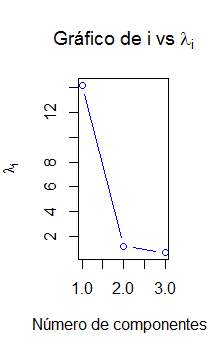
\includegraphics[width=0.4\textwidth]{img/Rplot1.png}
	\end{figure}
	
	
	\item \textbf{Desechar componentes asociados a valores propios inferiores a la cota:}
	
	\begin{lstlisting}
	cota<-sum(lambda)/9
	plot(	lambda, col = 4, type = "b", 
			main = TeX('$i$ vs $\lambda_i$'),
			xlab = TeX( '$i$'),
			ylab = TeX('$\lambda_i$')	)
	abline(h=cota, col= "red")
	\end{lstlisting}
	
	\item \textbf{Seleccionar componentes hasta cubrir una porción determinada de la
		varianza, como el 90\%}
	
	\begin{lstlisting}
	sum<-sum(E$values)
	sum
	# [1] 16.1
	Ve<-E$values/sum
	Ve
	# [1] 0.88129997 0.07401677 0.04468327
	sum_acu<-cumsum(Ve)
	sum_acu
	# 0.8813000 0.9553167 1.0000000
	\end{lstlisting}
	
	\begin{figure}
		\caption{Medidas de decisión}
		\centering
		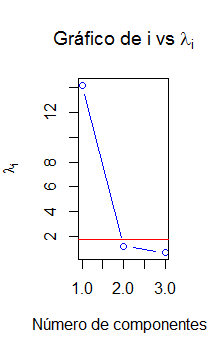
\includegraphics[width=0.4\textwidth]{img/Rplot2.png}
	\end{figure}
		
\end{itemize}

\section{Análisis de Componentes Principales con comando de R}

El programa estadístico \textbf{R} trae por defecto dos comando que realizan todos estos calculos y son los siguientes:

\subsection{prcomp()}

A este comando solo se le pasan los datos originales y de el obtenemos lo siguiente:

	\begin{lstlisting}
	acp_1<-prcomp(X)
	# Desviacion estandar de cada componente
	acp_1$sdev
	#[1] 3.7668195 1.0916364 0.8481749
	#La media de cada variable
	acp_1$center
	#[1] 5.166667 5.166667 5.166667
	#Los coeficientes de los componentes
	acp_1$rotation
	#            PC1        PC2        PC3
	# [1,] 0.7232056 -0.0704969  0.6870253
	# [2,] 0.6548975  0.3858469 -0.6497934
	# [3,] 0.2192782 -0.9198654 -0.3252149
	#Nuevas variables
	acp_1$x
	#             PC1          PC2        PC3
	# [1,] -3.5263639 -1.379315930 -1.0387069
	# [2,] -3.8966121  0.004071071  0.9485416
	# [3,] -1.2087140  1.091114870 -0.3138133
	# [4,] -0.4855084  1.020617969  0.3732121
	# [5,]  4.7422547  0.512784062 -0.8153154
	# [6,]  4.3749436 -1.249272041  0.8460819
	\end{lstlisting}
	
\subsection{primcomp()}

Al igual que el comando anterior sólo se necesita la matriz de datos. La forma de usarlo es la siguiente:

	\begin{lstlisting}
	acp_2<-princomp(X)
	#Desviacion estandar de cada componente
	acp_2$sdev
	#   Comp.1    Comp.2    Comp.3 
	# 3.4386201 0.9965231 0.7742742 
	#La media de cada variable
	acp_2$center
	# [1] 5.166667 5.166667 5.166667
	#Numero de observaciones
	acp_2$n.obs
	## [1] 6
	#Los coeficientes de los componentes
	acp$loadings
	# Loadings:
	#       Comp.1 Comp.2 Comp.3
	# [1,]  0.723         0.687
	# [2,]  0.655 -0.386 -0.650
	# [3,]  0.219  0.920 -0.325
	#                Comp.1 Comp.2 Comp.3
	# SS loadings     1.000  1.000  1.000
	# Proportion Var  0.333  0.333  0.333
	# Cumulative Var  0.333  0.667  1.000
	#Las nuevas variables
	acp_2$scores
	#          Comp.1       Comp.2     Comp.3
	# [1,] -3.5263639  1.379315930 -1.0387069
	# [2,] -3.8966121 -0.004071071  0.9485416
	# [3,] -1.2087140 -1.091114870 -0.3138133
	# [4,] -0.4855084 -1.020617969  0.3732121
	# [5,]  4.7422547 -0.512784062 -0.8153154
	# [6,]  4.3749436  1.249272041  0.8460819
	\end{lstlisting}

\section{Aplicación Web}

Para crear la aplicación web usaremos el paquete "\textbf{shiny}" del programa estadístico \textbf{R}. 

Una aplicación de \textbf{shiny} es una página web \textbf{ui} conectada a un computador que corre con una sesión de \textbf{R server}. 

La estructura es la siguiente: 

\begin{lstlisting}
library(shiny) 
ui <- fluidPage( ) 
server <- function( input, output){ } 
shinyApp( ui = ui, server = server) 
\end{lstlisting}

Los componentes de la aplicación son: 
\begin{itemize}
	\item \textbf{ui}: Aquí se presentan comandos de interfaz de usuario, en el se controla el diseño y aspecto de la aplicación. 
	\item \textbf{server}: Son los comandos del servidor, aquí se tienen las instrucciones que su equipo necesita para construir la aplicación.
	\item \textbf{shinyApp()}: Combina \textbf{ui} con \textbf{server} para crear la aplicación luego con \textbf{runApp()} se corre la aplicación. 
\end{itemize}

Para crear la aplicación se abre la consola de \textbf{R} y se crea un \textbf{script} con los componentes que acabamos de explicar y se guarda con el nombre de \textbf{app.R}

\chapter{Resultados}

\chapter{Conclusiones}

\chapter{Bibliografía}

\end{document}